\chapter{Results}
\label{ch:results}

All experiments in this chapter use the strict 70/20/10 subject-level split (3,611 training / 1,031 validation / 517 held-out test subjects), following the evaluation protocol established in the methodology chapter. Calibration samples are always the first K chronological segments of the target subject, and evaluation is performed on the subsequent five segments. The zero-shot baseline uses all 517 test subjects. The calibration-based methods require at least $K+5$ segments per subject, a condition met by 460 of the 517 test subjects at K=20; these therefore contribute $460 \times 5 = 2{,}300$ predictions, of which the number successfully parsed is reported as $n$.

\section{Cross-Subject Zero-Shot}

Table~\ref{tab:global} reports the zero-shot (global, no calibration) performance on the 517 held-out test subjects. A well-tuned XGBoost trained on 3,611 subjects achieves an MAE of SBP 15.7 mmHg and DBP 8.89 mmHg, failing every BHS grade: only 22.3\% of SBP errors fall within 5 mmHg, far below the 40\% required for Grade C. This is barely better than our earlier 857-subject pilot (SBP 17.0 mmHg), despite a four-fold increase in training data --- confirming that neither data quantity nor model capacity is the bottleneck.

For completeness, a preliminary LLM zero-shot experiment (no calibration samples, 20 subjects) yielded SBP 17.9 / DBP 14.6 --- comparable to the global XGBoost baseline and equally far from clinical usability. This confirms that the LLM, like conventional models, cannot generalise across subjects without personalisation.

\begin{table}[H]
\centering
\begin{tabular}{lcccc}
\toprule
Method & SBP MAE & DBP MAE & SBP BHS & DBP BHS \\
\midrule
XGBoost (global, 3,611 train) & 15.7 & 8.89 & --- & --- \\
\bottomrule
\end{tabular}
\caption{Global (zero-shot) XGBoost performance on 517 test subjects. ``---'' denotes failure of all BHS grades.}
\label{tab:global}
\end{table}

\section{Few-Shot Personalised Calibration}

\subsection{Calibration Ablation Across Methods}

Table~\ref{tab:ablation} summarises the K-ablation for all three personalised methods --- XGBoost bias correction, LLM numeric few-shot, and LLM semantic description. All methods improve as K increases, but the shape of improvement differs fundamentally.

\begin{table}[H]
\centering
\begin{tabular}{ccccc}
\toprule
K & XGBoost bias-corr & LLM numeric & LLM semantic & n (semantic) \\
\midrule
1 & 9.09 / 5.45 & 19.91 / 15.24 & 15.56 / 9.17 & 2,288 \\
3 & 8.28 / 4.83 & 12.74 / 8.65 & \textbf{8.23 / 4.56} & 2,052 \\
5 & 7.83 / 4.52 & 8.18 / 5.60 & \textbf{7.07 / 3.84} & 2,005 \\
10 & 7.27 / 3.99 & 6.59 / 4.11 & \textbf{5.84 / 3.16} & 1,988 \\
\textbf{20} & 7.79 / 4.18 & 5.99 / 3.32 & \textbf{5.52 / 2.93} & 1,910 \\
\bottomrule
\end{tabular}
\caption{K-ablation (SBP/DBP MAE in mmHg) on the 460 evaluated test subjects.}
\label{tab:ablation}
\end{table}

Two observations stand out. First, semantic description helps most when K is small: at K=1 it beats numeric few-shot by 4.4 mmHg on SBP (15.6 vs 19.9), and at K=3 by 4.5 mmHg (8.2 vs 12.7); the gap narrows to 0.5 mmHg at K=20. This is precisely the regime where the LLM most needs an external physiological prior. Second, XGBoost bias correction is comparatively flat across K, because it only estimates a constant offset rather than learning the individual mapping.

\subsection{Comparison with Conventional ML Calibration}

At K=20, LLM numeric few-shot achieves 5.99/3.32, outperforming XGBoost bias correction (7.79/4.18). This is a meaningful reversal of the picture suggested by our earlier 20-subject pilot, and reflects the much larger and more reliable test set. The LLM's in-context learning, given 20 calibration samples, genuinely adapts to the individual rather than merely shifting a population-level prediction.

\section{Full Comparison at K=20}

Table~\ref{tab:full_comparison} presents the complete comparison at K=20.

\begin{table}[H]
\centering
\begin{tabular}{lccc}
\toprule
Method & SBP MAE & DBP MAE & BHS grade (SBP / DBP) \\
\midrule
XGBoost (global) & 15.7 & 8.89 & --- / --- \\
XGBoost bias correction & 7.79 & 4.18 & C / A \\
LLM numeric few-shot & 5.99 & 3.32 & B / A \\
\textbf{LLM semantic description} & \textbf{5.52} & \textbf{2.93} & \textbf{B / A} \\
\bottomrule
\end{tabular}
\caption{Complete comparison at K=20 on the 460 evaluated test subjects.}
\label{tab:full_comparison}
\end{table}

Under the full BHS cumulative protocol, the semantic method reaches Grade A for DBP (84.0\% of errors $\leq$5 mmHg, 95.3\% $\leq$10, 98.6\% $\leq$15) and Grade B for SBP (63.2\% $\leq$5, 85.0\% $\leq$10, 92.3\% $\leq$15), as shown in Table~\ref{tab:bhs}. The SBP distribution is on the boundary of Grade A, falling short only on the $\leq$15 mmHg criterion.

\begin{table}[H]
\centering
\begin{tabular}{lcccc}
\toprule
Target & $\leq$5 mmHg & $\leq$10 mmHg & $\leq$15 mmHg & Grade \\
\midrule
SBP & 63.2\% & 85.0\% & 92.3\% & B \\
DBP & 84.0\% & 95.3\% & 98.6\% & A \\
\bottomrule
\end{tabular}
\caption{BHS cumulative error distribution of semantic description at K=20.}
\label{tab:bhs}
\end{table}

\begin{figure}[H]
\centering
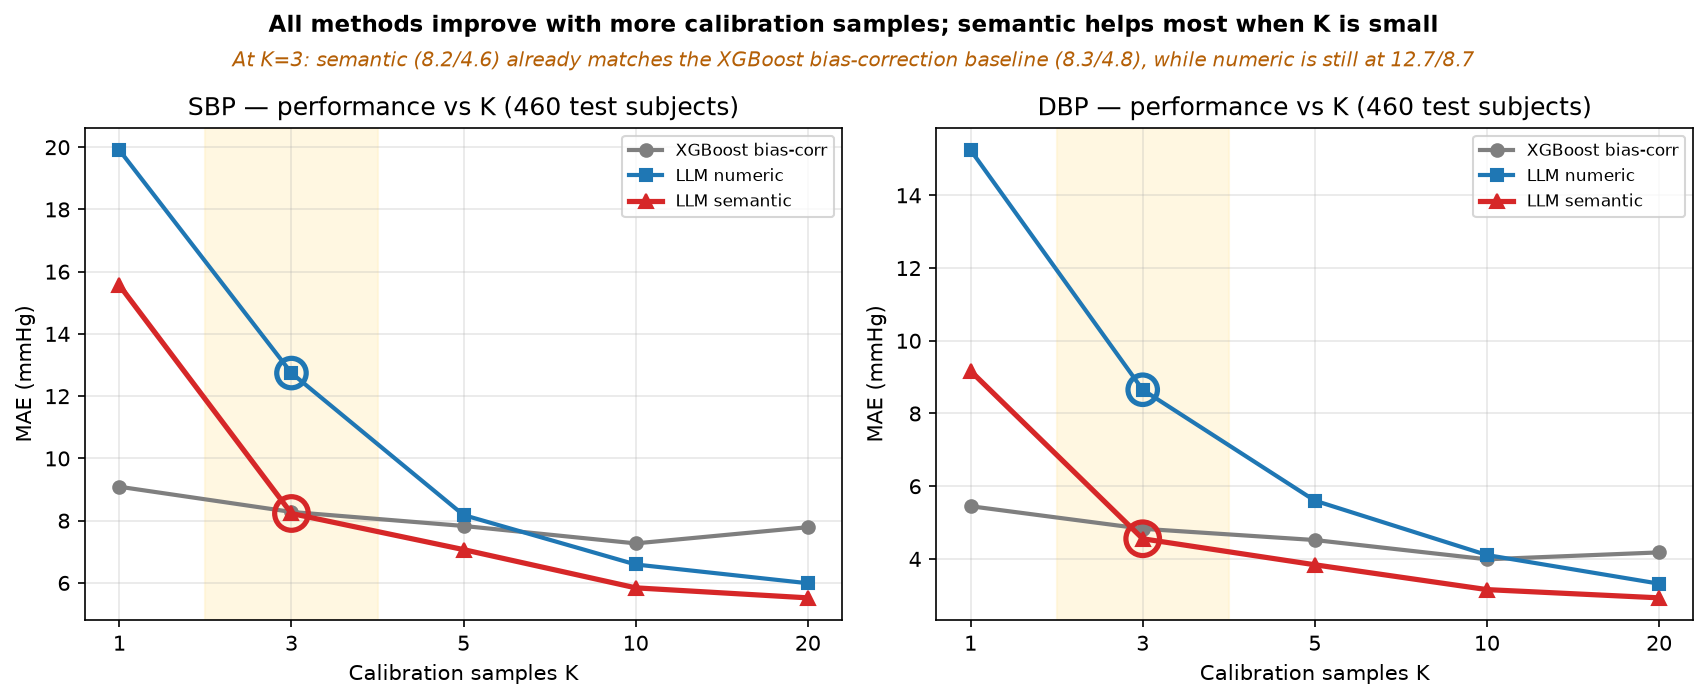
\includegraphics[width=0.95\textwidth]{figures/fig_k_ablation.png}
\caption{K-ablation curves for all three methods on the 460 evaluated test subjects. The shaded band highlights K=3, where semantic description already matches the XGBoost bias-correction baseline.}
\label{fig:k_ablation}
\end{figure}

\begin{figure}[H]
\centering
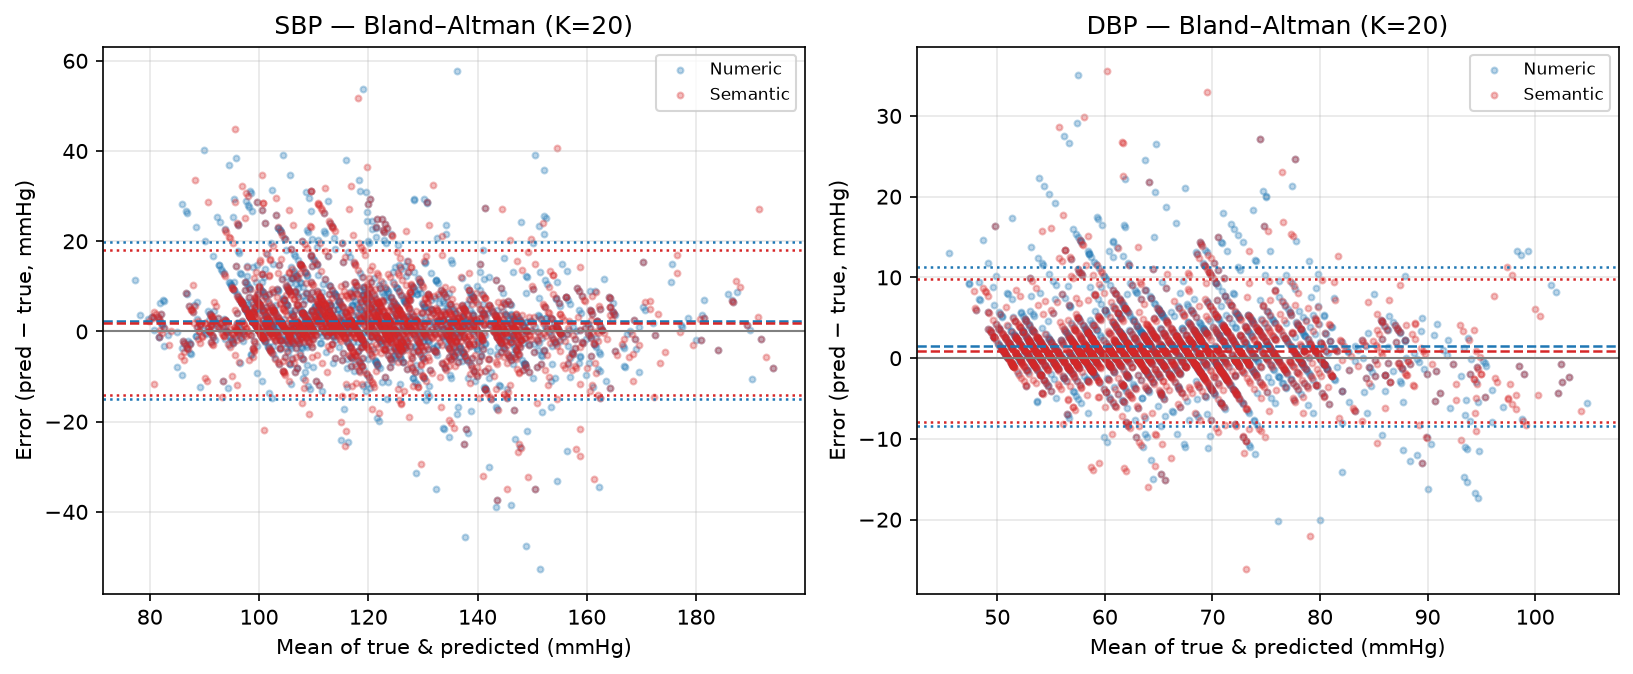
\includegraphics[width=0.95\textwidth]{figures/fig_numeric_vs_semantic.png}
\caption{Bland--Altman comparison of numeric few-shot and semantic description at K=20.}
\label{fig:bland_altman}
\end{figure}

\section{Validation-Set Hyperparameter Tuning}

To ensure the 70/20/10 validation set (1,031 subjects) is used for its intended purpose, we ran a nine-combination grid search over XGBoost hyperparameters (three max-depths $\times$ three learning rates). The validation MAE varied by less than 0.2 mmHg across all combinations, and the best combination performed almost identically to our default settings on the test set (differences up to 0.15 mmHg). We therefore retained the default settings, which also confirms that the reported results are robust to hyperparameter choice.

\section{Semantic Bottleneck}

As a negative control, a purely qualitative semantic bottleneck --- which discards all quantitative anchors --- achieves only SBP 25.0 / DBP 23.5 (preliminary, 20 subjects). This is far worse than every other method, confirming that language helps only when it carries quantitative information: purely qualitative summaries make precise regression impossible. This control is qualitative in nature and does not depend on the split size, so it was not re-run on the 517-subject test set.
